\documentclass{beamer}

\usetheme{CambridgeUS}

\usepackage[greek]{babel}
\usepackage{multirow}
\usepackage{booktabs}

\newcommand{\gr}{\selectlanguage{greek}}
\newcommand{\en}{\selectlanguage{english}}


%Information to be included in the title page:
\title[Ομάδα 30] 
{Εργασία Αναγνώρησης Προτύπων και Μηχανικής Μάθησης}


\author[Βασίλης Αϊτσίδης, Φίλιππος Ρωσσίδης]
{Βασίλης Αϊτσίδης (10330) \\ Φίλιππος Ρωσσίδης (10379) \\ Ομάδα 30}

\institute{ΑΠΘ}

\date{\today}

\begin{document}

\frame{\titlepage}

\AtBeginSection[]
{
  \begin{frame}
    \frametitle{Πίνακας Περιεχομένων}
    \tableofcontents[currentsection]
  \end{frame}
}

\section{ΜΕΡΟΣ Α - Εκτίμηση με Μέγιστη Πιθανοφάνεια}

\begin{frame}
\frametitle{Εκτίμηση με Μέγιστη Πιθανοφάνεια}

Υποθέτουμε ότι έχουμε δείγματα μιας τιμής $x$ για τα οποία θέλουμε να
αναλύσουμε κατά πόσο είναι αξιόπιστοι δείκτες του στρες για παίκτες βιντεπαιχνιδιών.

Γνωρίζουμε ότι η ΣΠΠ του $x$ είναι: 
$p(x|\theta) = \frac{1}{\pi} \frac{1}{1+(x-\theta)^2}$, όπου το $\theta$ 
είναι άγνωστο. 

Γνωρίζουμε επίσης ότι από σύνολο 12 δεδομένων: για 7 παίκτες που δεν ένιωσαν στρες (κλάση $\omega_1$)
οι δείκτες $x$ ήταν $D_1=[ 2.8, -0.4, -0.8, 2.3,-0.3,3.6,4.1]$, ενώ για τους 5 παίκτες
που ένιωσαν στρες 
οι δείκτες $x$ ήταν $D_2=[-4.5,-3.4,-3.1,-3.0,-2.3]$. 


Για να βρούμε εάν είναι αξιόπιστος ο δείκτης $x$ θα προσπαθήσουμε να βρούμε τρόπο
να ταξινομούμε κάποιον παίκτη σε κλάσεις: στρες, όχι στρες, με τη χρήση του 
δείκτη $x$. 

Στο πρώτο μέρος θα χρησιμοποιήσουμε τη μέθοδο Μέγιστης Πιθανοφάνειας.

\end{frame}



\begin{frame}
\frametitle{Εκτίμηση με Μέγιστη Πιθανοφάνεια}

Αρχικά μπορούμε να παρατηρήσουμε (και με μια οπτικοποίηση στο σχήμα \ref{fig:1}): ότι 
οι δύο κλάσεις (για τα δείγματα που έχουμε) είναι γραμμικά διαχωρίσημες, άρα 
ήδη μπορούμε να συμπεράνουμε ότι το $x$ θα έχει σχετικά αξιόπιστα αποτελέσματα.

\begin{figure}
    \centering
        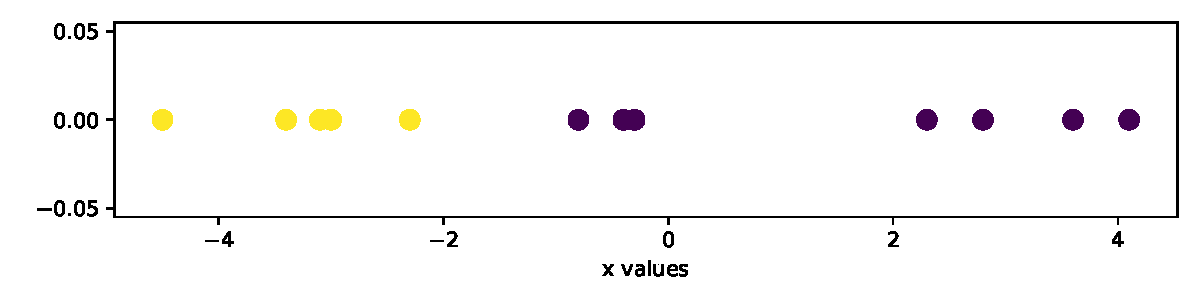
\includegraphics[width=0.7\textwidth]{./plots/Figure_1.pdf}
        \caption{Οι τιμές των δειγμάτων. Κίτρινο=στρες, μωβ=οχι στρες}
        \label{fig:1}
\end{figure}



\end{frame}


\begin{frame}
\frametitle{Εκτίμηση με Μέγιστη Πιθανοφάνεια}

Εκτιμάμε τις παραμέτρους $\hat{\theta_1}, \hat{\theta_2}$ των ΣΠΠ και για τις δύο 
κλάσεις, δηλαδή τις τιμές που μεγιστοποιούν τις (συναρτήσεις πιθανοφάνειας) $p(D_1|\theta)$ και $p(D_2|\theta)$,
αντίστοιχα.

Εκτελούμε τα παρακάτω βήματα για διάφορες τιμές του $\theta$:

\begin{itemize}
    \item $p(x|\theta) = \frac{1}{\pi} \frac{1}{1+(x-\theta)^2}$
    \item $p(D|\theta) = p(x_1, x_2, \dots, x_N | \theta) = \prod_{n=1}^N p(x_n | \theta)$
 
\end{itemize}
 
Βρίσκουμε την τιμή $\hat{\theta}$ που μεγιστοποιεί  το $p(D|\theta)$.

Στην υλοποίηση επιλέχθηκαν 500 τιμές για το $\theta$ στο διάστημα $[-60,60]$.


\end{frame}

\begin{frame}
\frametitle{Εκτίμηση με Μέγιστη Πιθανοφάνεια}

\begin{columns}

    \column{0.5\textwidth}
    
    Δεξιά παρατίθονται οι συναρτήσεις πιθανοφάνειας $p(D|\theta)$ για τις 
    δύο κλάσεις. Οι τιμές του $\theta$ που τις μεγιστοποιούν είναι η Εκτίμηση
    του αλγορίθμου. Συγκεκριμένα για τα δεδομένα που έχουμε, οι τιμές είναι:
    $\theta_1 = 2.525, \theta_2 = -3.246$.

    Επίσης, να σημειωθεί ότι όσο περισσότερα είναι τα δείγματα, τόσο πιο 
    στενή θα είναι η καμπύλη $p(D|\theta)$.


    \column{0.5\textwidth}

    \begin{figure}
        \centering
            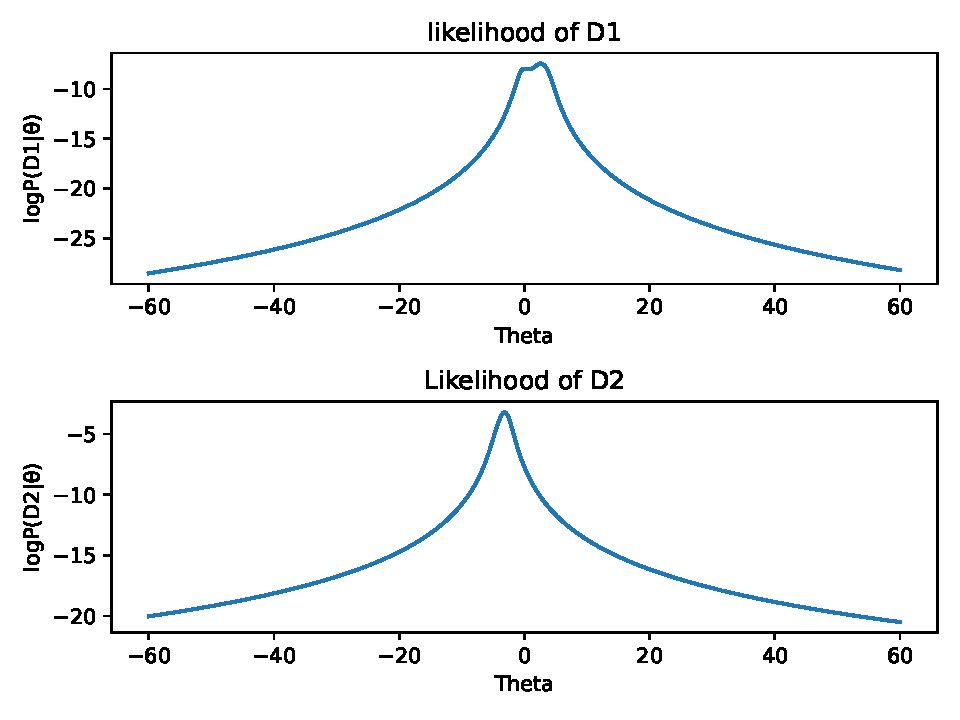
\includegraphics[width=\textwidth]{./plots/likelihoods.pdf}
            \caption{Συναρτήσεις πιθανοφάνειας για τις δύο κλάσεις.}
            \label{fig:likelihoods}
    \end{figure}


\end{columns}


    

\end{frame}



\begin{frame}
    \frametitle{Εκτίμηση με Μέγιστη Πιθανοφάνεια}
    
    Προκειμένου να ταξινομήσουμε τα $x$ σε κλάσεις χρησιμοποιούμε την συνάρτηση διάκρισης:
    \[g(x) = \log P(x | \hat{\theta}_1) - \log P(x | \hat{\theta}_2) + \log P(\omega_1) - \log P(\omega_2)\]

    Η συνάρτηση αυτή προκύπτει από τον γενικό κανόνα του Μπεϋζ $GBR$: 
    \[\frac{p(\mathbf{x} \mid \omega_1)}{p(\mathbf{x} \mid \omega_2)} > \frac{\lambda_{12} - \lambda_{22}}{\lambda_{21} - \lambda_{11}} \frac{P(\omega_2)}{P(\omega_1)} \]
    με θεωρήσεις:

    \begin{itemize}
        \item $\lambda_{11} = \lambda_{22} = 0$, δηλαδή η ποινή σωστής ταξινόμησης είναι 0.
        \item $\lambda_{12} = \lambda_{21} = 1$, δηλαδή η ποινή λανθασμένης ταξινόμησης είναι 1.
    \end{itemize}

    αν λογαριθμίσουμε και τις δύο πλευρές.

    $g(x) > 0 \Rightarrow P(\omega_1|x) > P(\omega_2|x)$, αρά κατατάσουμε το $x$ στην $\omega_1$.
    Διαφορετικά $g(x) < 0 \Rightarrow P(\omega_1|x) <  P(\omega_2|x)$ , αρά κατατάσουμε το $x$ στην $\omega_2$.

    
\end{frame}


\begin{frame}{Εκτίμηση με Μέγιστη Πιθανοφάνεια}
    \begin{columns} % Begin columns
        % First column: Text
        \begin{column}{0.48\textwidth}
            \textbf{Παρατηρήσεις}
            \begin{itemize}
                \item Οι τιμές της \( g(x) \) καθορίζουν την κλάση.
                \item Θετικές τιμές της \( g(x) \) αντιστοιχούν στην κλάση \( \omega_1 \).
                \item Αρνητικές τιμές της \( g(x) \)αντιστοιχούν στην κλάση \( \omega_2 \).
                \item Με μία εξαίρεση την τιμή $x=-0.8$ όπου η $g(x)$ είναι αρνητική, αλλά το 
                δείγμα ανήκει στην κλάση \( \omega_1 \).
            \end{itemize}
        \end{column}

        % Second column: Table
        \begin{column}{0.48\textwidth}
            \centering
            \resizebox{0.85\textwidth}{!}{%
                \begin{tabular}{rrl}
                    \toprule
                    \( x \) & \( g(x) \) & Κλάση \\
                    \midrule
                    2.8  & 1.689205  & \( \omega_1 \) \\
                    -0.4 & 0.125017  & \( \omega_1 \) \\
                    -0.8 & -0.090887 & \( \omega_1 \) \\
                    2.3  & 1.626600  & \( \omega_1 \) \\
                    -0.3 & 0.178765  & \( \omega_1 \) \\
                    3.6  & 1.492680  & \( \omega_1 \) \\
                    4.1  & 1.344624  & \( \omega_1 \) \\
                    -4.5 & -1.145734 & \( \omega_2 \) \\
                    -3.4 & -1.401339 & \( \omega_2 \) \\
                    -3.1 & -1.358416 & \( \omega_2 \) \\
                    -3.0 & -1.326927 & \( \omega_2 \) \\
                    -2.3 & -0.961337 & \( \omega_2 \) \\
                    \bottomrule
                \end{tabular}
            }
        \end{column}
    \end{columns}
\end{frame}




\begin{frame}{Εκτίμηση με Μέγιστη Πιθανοφάνεια}
    \begin{figure}
        \centering
            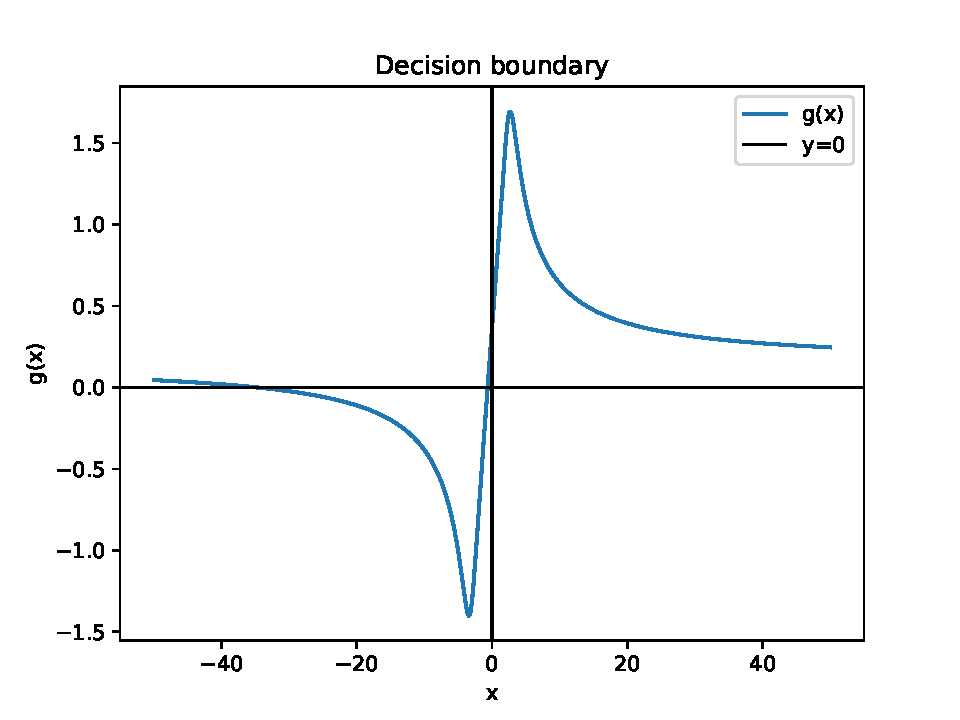
\includegraphics[width=0.6\textwidth]{./plots/DB1.pdf}
            \caption{$g(x)$ ως προς $x$. Φαίνονται οι περιοχές απόφασης του αλγορίθμου. Αν 
            η $g(x)$ είναι θετική αποφασίζουμε $\omega_1$, αλλιώς $\omega_2$. Όπως προαναφέρθηκε, 
            για $x=-0.8$ η απόφαση είναι λανθασμένη.}
            \label{fig:DB1}
    \end{figure}

    
\end{frame}



\section{ΜΕΡΟΣ Β - Μπεϋζιανή Εκτίμηση}

\begin{frame}
    \frametitle{ΜΕΡΟΣ Β}
    
    
\end{frame}




\section{ΜΕΡΟΣ Γ - Ίριδα (Δέντρο Απόφασης/ Τυχαίο Δάσος)}
\begin{frame}
    \frametitle{ΜΕΡΟΣ Γ}
    
    
\end{frame}




\section{ΜΕΡΟΣ Δ}

\begin{frame}
    \frametitle{ΜΕΡΟΣ Δ}
    
    
\end{frame}



\end{document}